\chapter{अंतराआण्विक बल और विलायक}\label{ch:b1:intermolecular-forces-solvents}

छिपकली खिड़की के काँच पर दौड़ती हुई चढ़ जाती है और एक उँगली के सहारे उससे लटकी
रहती है; न कोई गोंद, न चूषण, केवल उसके पंजों की गद्दियों के अणुओं और काँच के अणुओं
के बीच का आकर्षण। पानी, जिसका अणु कार्बन डाइऑक्साइड से हल्का है,
\qty{100}{\celsius} पर उबलता है, जबकि कार्बन डाइऑक्साइड कमरे के ताप पर
गैस है। तेल सिरके पर तैरता है और उसमें कभी नहीं मिलता; खाने का
नमक पानी में घुलता है, पेट्रोल में नहीं। ये सब तथ्य अणुओं के भीतर के आबंध
तय नहीं करते, बल्कि उनके बीच के कहीं अधिक दुर्बल बल। यह अध्याय उन बलों का
वर्गीकरण करता है, क्वथनांकों पर उनके प्रभाव मापता है, और उनकी सहायता से विलायक चुनता है।

% ledger: bp:H2O (the hook's 100 degC)

\begin{recall}
पुस्तक 1 (कक्षा 11) ने वान्डरवाल्स बलों और \omterm{def:b1:intermolecular-forces-solvents:hbond}{हाइड्रोजन आबंधों} का परिचय दिया था,
और समझाया था कि आयनिक ठोस वियोजन और \omterm{def:b1:intermolecular-forces-solvents:dissolution}{विलायकन} द्वारा घुलते हैं।
\omterm{def:b1:lewis-resonance-vsepr:dipole}{द्विध्रुव आघूर्णों} की परिभाषा \cref{def:b1:lewis-resonance-vsepr:dipole} में
और \omterm{def:b1:periodicity:polarisability}{ध्रुवणीयता} की \cref{def:b1:periodicity:polarisability} में दी गई। भौतिकी
से हम कूलॉम का नियम लेते हैं: दो आवेश $q_1$ और $q_2$, निर्वात में दूरी $r$ पर,
एक-दूसरे को $|q_1q_2|/(4\pi
\varepsilon_0 r^2)$ मान के बल से आकर्षित या प्रतिकर्षित करते हैं।
\end{recall}

\begin{omfigure}
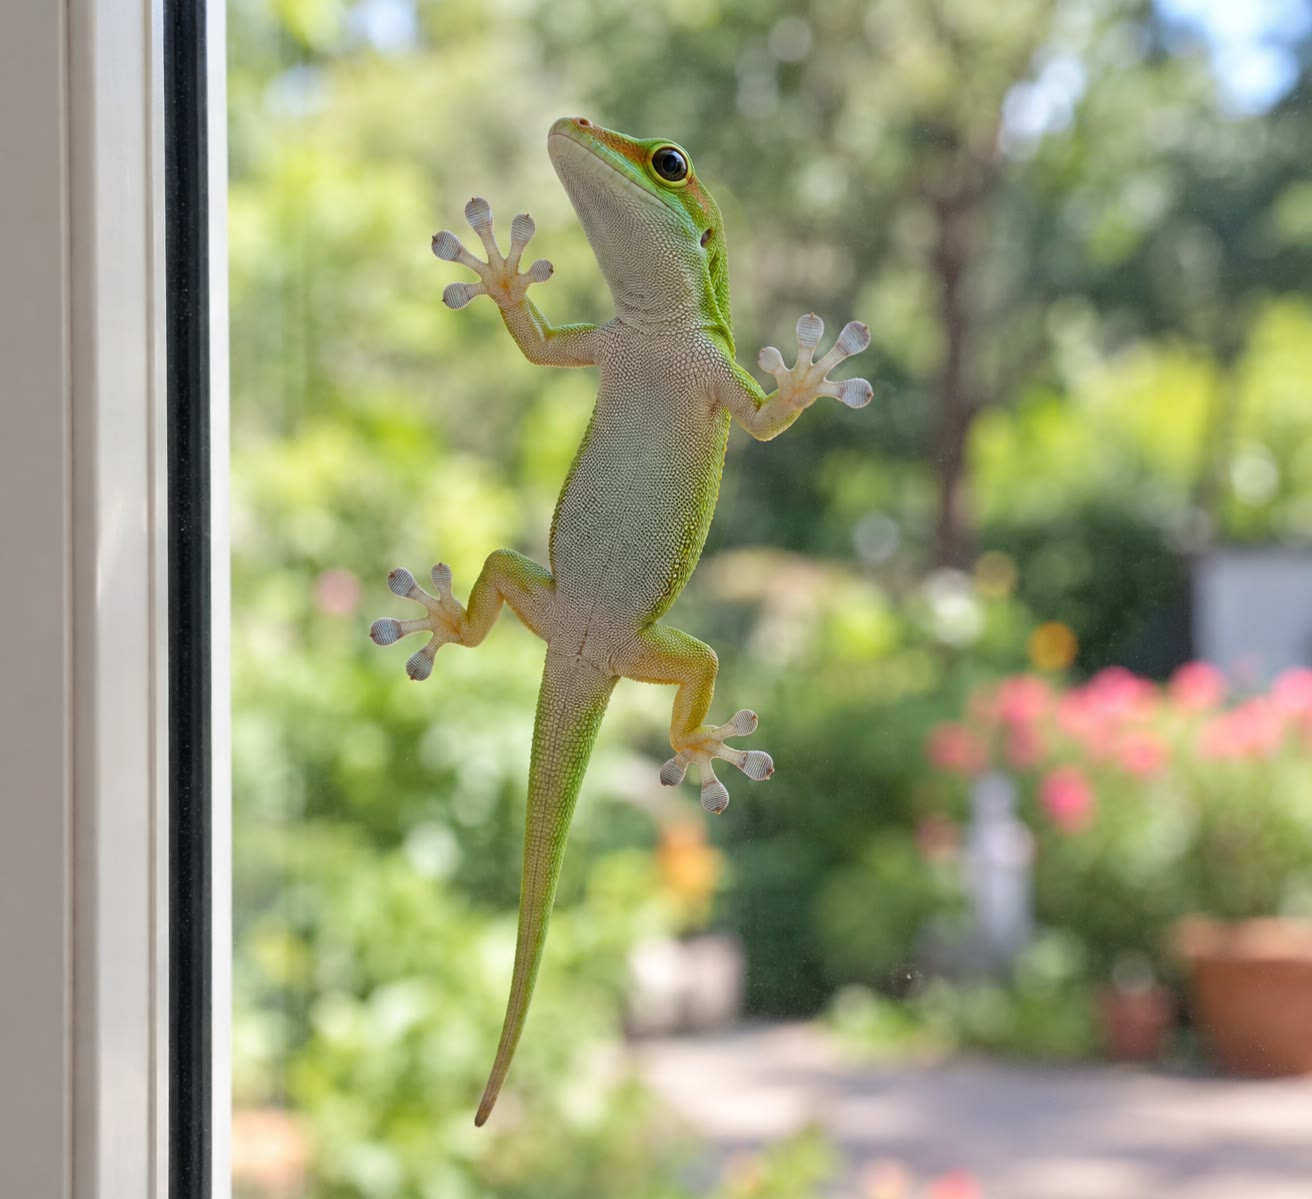
\includegraphics[width=0.52\linewidth]{images/book2/ai/b1-04-gecko.jpg}

{\small खिड़की के काँच पर एक छिपकली। उसके पंजों की गद्दियों के लाखों बारीक रोम
काँच के इतने पास आ जाते हैं कि उनके अणुओं और काँच के अणुओं के बीच का
दुर्बल आकर्षण जुड़कर उसके भार से अधिक हो जाता है।}
\end{omfigure}

\section{वान्डरवाल्स अन्योन्यक्रियाएँ}

\begin{definition}[वान्डरवाल्स अन्योन्यक्रियाएँ]\label{def:b1:intermolecular-forces-solvents:vdw}
\emph{वान्डरवाल्स अन्योन्यक्रियाएँ}\index{वान्डरवाल्स अन्योन्यक्रिया}
उदासीन अणुओं के बीच के वे आकर्षण हैं जो उनके द्विध्रुवों की
अन्योन्यक्रिया से उत्पन्न होते हैं। तीन प्रकार पहचाने जाते हैं:
\begin{itemize}
  \item \emph{कीसोम अन्योन्यक्रिया}\index{कीसोम अन्योन्यक्रिया} (या
        अभिविन्यास अन्योन्यक्रिया), दो स्थायी द्विध्रुवों के बीच, जो
        सिर से पूँछ की ओर संरेखित होने की प्रवृत्ति रखते हैं;
  \item \emph{डिबाई अन्योन्यक्रिया}\index{डिबाई अन्योन्यक्रिया} (या
        प्रेरण अन्योन्यक्रिया), किसी स्थायी द्विध्रुव और उस द्विध्रुव के बीच
        जिसे वह किसी ध्रुवणीय पड़ोसी में प्रेरित करता है;
  \item \emph{लंदन अन्योन्यक्रिया}\index{लंदन अन्योन्यक्रिया} (या
        परिक्षेपण अन्योन्यक्रिया), उन क्षणिक द्विध्रुवों के बीच जो
        इलेक्ट्रॉन मेघों के उतार-चढ़ाव किन्हीं भी दो परमाणुओं या
        अणुओं में, ध्रुवीय हों या नहीं, उत्पन्न करते हैं और जो एक-दूसरे को प्रेरित करते हैं।
\end{itemize}
\end{definition}

\begin{omfigure}
\begin{tikzpicture}[font=\small, >={Stealth},
    mol/.style={draw=black!60, fill=#1, ellipse, minimum width=1.5cm, minimum height=0.8cm}]
  % Keesom
  \node[mol=omDef!20] (a) at (0,0) {}; \node[mol=omDef!20] (b) at (1.7,0) {};
  \node at (-0.45,0) {$\delta^-$}; \node at (0.45,0) {$\delta^+$};
  \node at (1.25,0) {$\delta^-$}; \node at (2.15,0) {$\delta^+$};
  \node[below, align=center] at (0.85,-0.65) {कीसोम:\\दो स्थायी द्विध्रुव};
  % Debye
  \begin{scope}[xshift=4.6cm]
    \node[mol=omDef!20] at (0,0) {}; \node[mol=black!5, dashed] at (1.7,0) {};
    \node at (-0.45,0) {$\delta^-$}; \node at (0.45,0) {$\delta^+$};
    \node[omProp] at (1.25,0) {$\delta^-$}; \node[omProp] at (2.15,0) {$\delta^+$};
    \node[below, align=center] at (0.85,-0.65) {डिबाई:\\स्थायी और प्रेरित};
  \end{scope}
  % London
  \begin{scope}[xshift=9.2cm]
    \node[mol=black!5, dashed] at (0,0) {}; \node[mol=black!5, dashed] at (1.7,0) {};
    \node[omProp] at (-0.45,0) {$\delta^-$}; \node[omProp] at (0.45,0) {$\delta^+$};
    \node[omProp] at (1.25,0) {$\delta^-$}; \node[omProp] at (2.15,0) {$\delta^+$};
    \node[below, align=center] at (0.85,-0.65) {लंदन:\\दो क्षणिक द्विध्रुव};
  \end{scope}
\end{tikzpicture}

{\small तीनों \omterm{def:b1:intermolecular-forces-solvents:vdw}{वान्डरवाल्स अन्योन्यक्रियाएँ}। काले आंशिक आवेश
स्थायी हैं (\omterm{def:b1:lewis-resonance-vsepr:dipole}{ध्रुवीय अणु}); नारंगी आवेश प्रेरित या क्षणिक हैं।
हर स्थिति में आमने-सामने के आवेश विपरीत हैं, इसलिए अणु
एक-दूसरे को आकर्षित करते हैं।}
\end{omfigure}

\begin{proposition}[सामर्थ्य और परास]\label{prop:b1:intermolecular-forces-solvents:distance-law}
दूरी $r$ पर स्थित दो अणुओं के लिए तीनों वान्डरवाल्स
ऊर्जाओं में से हर एक $-1/r^6$ के अनुसार बदलती है: आकर्षण केवल पड़ोसियों के बीच
अनुभव होता है। इनकी ऊर्जाएँ कुछ किलोजूल प्रति मोल की कोटि की होती हैं,
\omterm{def:b1:lewis-resonance-vsepr:lewis}{सहसंयोजी आबंध} से लगभग सौ गुना कम। लंदन पद
दोनों साथियों की \omterm{def:b1:periodicity:polarisability}{ध्रुवणीयताओं} के साथ बढ़ता है; यह
सभी अणुओं के बीच मौजूद होता है और प्रायः तीनों में सबसे बड़ा होता है, छोटे,
अत्यधिक \omterm{def:b1:lewis-resonance-vsepr:dipole}{ध्रुवीय अणुओं} को छोड़कर।
\end{proposition}
\admitted

\begin{example}[उत्कृष्ट गैसें और हैलोजन]\label{ex:b1:intermolecular-forces-solvents:noble}
किसी उत्कृष्ट गैस के परमाणु एक-दूसरे को केवल लंदन बलों से आकर्षित करते हैं,
जो इलेक्ट्रॉनों की संख्या के साथ बढ़ते हैं: हीलियम
\qty{-268.9}{\celsius} पर उबलती है, नियॉन \qty{-246.1}{\celsius} पर, आर्गन
\qty{-185.9}{\celsius} पर, क्रिप्टॉन \qty{-153.4}{\celsius} पर, ज़ेनॉन
\qty{-108.1}{\celsius} पर। इसी तरह, कमरे के ताप पर, डाइफ़्लुओरीन और
डाइक्लोरीन गैसें हैं, डाइब्रोमीन द्रव (\qty{58.8}{\celsius} पर उबलने वाला)
और डाइआयोडीन ठोस।
% ledger: bp:He, bp:Ne, bp:Ar, bp:Kr, bp:Xe, bp:F2, bp:Cl2, bp:Br2, bp:I2
\end{example}

\begin{omfigure}
\begin{tikzpicture}
\begin{axis}[
  width=0.62\linewidth, height=5.4cm,
  xmin=0.5, xmax=10.5, ymin=-180, ymax=200,
  axis x line=bottom, axis y line=left,
  xlabel={कार्बन परमाणुओं की संख्या $n$}, ylabel={क्वथनांक (\unit{\celsius})},
  xtick={1,2,3,4,5,6,7,8,9,10}, ytick={-150,-100,-50,0,50,100,150},
  tick label style={font=\small}, label style={font=\small}]
\addplot[omDef, thick, mark=*, mark size=1.5pt] table[x=n, y=bp_C] {figdata/out/bachelor-1-hydride-boiling-points-alkanes.dat};
\end{axis}
\end{tikzpicture}

{\small रैखिक ऐल्केनों \ce{C_nH_{2n+2}} के क्वथनांक, मेथेन से
डेकेन तक। जुड़ने वाला हर \ce{CH2} इलेक्ट्रॉन और संपर्क-सतह जोड़ता है, अतः
लंदन आकर्षण भी; वृद्धि धीरे-धीरे घटती है, आरंभ में लगभग
\qty{75}{\celsius} से डेकेन पर \qty{25}{\celsius} तक।}
\end{omfigure}

\section{हाइड्रोजन आबंध}

\begin{definition}[हाइड्रोजन आबंध]\label{def:b1:intermolecular-forces-solvents:hbond}
\emph{हाइड्रोजन आबंध}\index{हाइड्रोजन आबंध} एक आकर्षण
$\ce{X-H}\cdots\ce{Y}$ है, जो किसी छोटे, अत्यधिक
विद्युत-ऋणात्मक परमाणु X (\ce{N}, \ce{O} या \ce{F}) से आबंधित हाइड्रोजन परमाणु और
किसी दूसरे विद्युत-ऋणात्मक परमाणु Y के \omterm{def:b1:lewis-resonance-vsepr:lewis}{एकाकी युग्म} के बीच होता है। जिस अणु पर \ce{X-H} है वह
हाइड्रोजन-आबंध दाता है, जिस पर Y है वह ग्राही। इसकी ऊर्जा, 10
से \qty{40}{kJ/mol}, \omterm{def:b1:intermolecular-forces-solvents:vdw}{वान्डरवाल्स अन्योन्यक्रियाओं} और \omterm{def:b1:lewis-resonance-vsepr:lewis}{सहसंयोजी
आबंधों} के बीच है; तीनों परमाणु \ce{X}, \ce{H}, \ce{Y} लगभग एक रेखा में होते हैं।
\end{definition}

\begin{remark}[N, O और F ही क्यों]\label{rem:b1:intermolecular-forces-solvents:why}
प्रबल विद्युत-ऋणात्मक X हाइड्रोजन पर बड़ा आंशिक
धनात्मक आवेश छोड़ता है; हाइड्रोजन, जिसके पास कोई भीतरी इलेक्ट्रॉन नहीं, बहुत छोटा है, इसलिए
Y का \omterm{def:b1:lewis-resonance-vsepr:lewis}{एकाकी युग्म} उसके बहुत पास आ सकता है। दोनों शर्तें आवश्यक हैं:
\ce{C-H} आबंध पर्याप्त ध्रुवीय नहीं हैं, और \ce{S-H} या \ce{Cl-H} आबंधों में
ऐसे परमाणु होते हैं जो प्रबल \omterm{def:b1:intermolecular-forces-solvents:hbond}{हाइड्रोजन आबंध} बनाने के लिए बहुत बड़े और बहुत कम
विद्युत-ऋणात्मक हैं।
\end{remark}

\begin{omfigure}
\begin{tikzpicture}[font=\small]
  % water network
  \foreach \n/\x/\y/\a in {1/0/0/0, 2/2.2/0.9/200, 3/0.2/-2.0/60, 4/-2.1/0.6/-30} {
    \begin{scope}[shift={(\x,\y)}, rotate=\a]
      \node[aO] (o\n) at (0,0) {};
      \node[aH] (h\n a) at (0.78,0.3) {};
      \node[aH] (h\n b) at (-0.2,-0.82) {};
      \begin{scope}[on background layer]
        \draw[bond] (o\n.center) -- (h\n a.center); \draw[bond] (o\n.center) -- (h\n b.center);
      \end{scope}
    \end{scope}
  }
  \draw[omThm, thick, densely dotted] (h1a) -- (o2);
  \draw[omThm, thick, densely dotted] (h1b) -- (o3);
  \draw[omThm, thick, densely dotted] (h4a) -- (o1);
  \node[below] at (0,-2.9) {पानी: हर अणु दो दे सकता है और दो ले सकता है};
  % carboxylic acid dimer
  \begin{scope}[xshift=5.6cm, yshift=-0.6cm]
    \node (r1) at (-0.9,0) {R}; \node (c1) at (0,0) {C};
    \node (o1) at (0.6,0.85) {O}; \node (o2) at (0.6,-0.85) {O}; \node (h2) at (1.45,-0.85) {H};
    \node (c2) at (3.3,0) {C}; \node (r2) at (4.2,0) {R};
    \node (o3) at (2.7,0.85) {O}; \node (o4) at (2.7,-0.85) {O}; \node (h3) at (1.85,0.85) {H};
    \draw (r1) -- (c1) -- (o2) -- (h2) (c2) -- (r2) (c2) -- (o3) -- (h3);
    \draw[double, double distance=1.6pt] (c1) -- (o1); \draw[double, double distance=1.6pt] (c2) -- (o4);
    \draw[omThm, thick, densely dotted] (h2) -- (o4) (h3) -- (o1);
    \node[below] at (1.65,-2.3) {कार्बोक्सिलिक अम्ल का द्वितय};
  \end{scope}
\end{tikzpicture}

{\small \omterm{def:b1:intermolecular-forces-solvents:hbond}{हाइड्रोजन आबंध} (लाल बिंदुदार)। द्रव पानी में हर अणु अधिकतम चार
\omterm{def:b1:intermolecular-forces-solvents:hbond}{हाइड्रोजन आबंधों} में भाग लेता है; कार्बोक्सिलिक अम्ल चक्रीय द्वितयों में
जोड़े बनाते हैं, जिन्हें दो \omterm{def:b1:intermolecular-forces-solvents:hbond}{हाइड्रोजन आबंध} थामे रहते हैं।}
\end{omfigure}

\begin{proposition}[हाइड्रोजन आबंध क्वथनांक बढ़ाते हैं]\label{prop:b1:intermolecular-forces-solvents:hbond-bp}
\omterm{def:b1:periodicity:table}{समूह} 15, 16 और 17 के हाइड्राइडों में क्वथनांक
\omterm{def:b1:periodicity:table}{आवर्त} 3 से \omterm{def:b1:periodicity:table}{आवर्त} 5 तक बढ़ता है, \omterm{def:b1:intermolecular-forces-solvents:vdw}{लंदन अन्योन्यक्रिया} का अनुसरण करते हुए;
\omterm{def:b1:periodicity:table}{आवर्त} 2 के हाइड्राइड \ce{NH3}, \ce{H2O} और \ce{HF}, जो \omterm{def:b1:intermolecular-forces-solvents:hbond}{हाइड्रोजन
आबंध} बनाते हैं, उस प्रवृत्ति के बहिर्वेशन से कहीं ऊपर उबलते हैं। \omterm{def:b1:periodicity:table}{समूह} 14 के
हाइड्राइड (\ce{CH4}, \ce{SiH4}, \ce{GeH4}) कोई \omterm{def:b1:intermolecular-forces-solvents:hbond}{हाइड्रोजन आबंध} नहीं बनाते और
प्रवृत्ति का पालन करते हैं।
\end{proposition}

\begin{omfigure}
\begin{tikzpicture}
\begin{axis}[
  width=0.82\linewidth, height=6.6cm,
  xmin=1.5, xmax=5.6, ymin=-180, ymax=120,
  axis x line=bottom, axis y line=left,
  xlabel={आवर्त}, ylabel={क्वथनांक (\unit{\celsius})},
  xtick={2,3,4,5}, ytick={-150,-100,-50,0,50,100},
  tick label style={font=\small}, label style={font=\small},
  clip=false]
\addplot[black!60, thick, mark=square*, mark size=1.6pt] table[x=period, y=bp_C] {figdata/out/bachelor-1-hydride-boiling-points-g14.dat};
\addplot[omDef, thick, mark=*, mark size=1.6pt] table[x=period, y=bp_C] {figdata/out/bachelor-1-hydride-boiling-points-g15.dat};
\addplot[omThm, thick, mark=*, mark size=1.6pt] table[x=period, y=bp_C] {figdata/out/bachelor-1-hydride-boiling-points-g16.dat};
\addplot[omMeth, thick, mark=triangle*, mark size=2pt] table[x=period, y=bp_C] {figdata/out/bachelor-1-hydride-boiling-points-g17.dat};
\addplot[omThm, dashed] coordinates {(2,-79.3) (3,-60.3)};
\node[font=\small, anchor=west] at (axis cs:2.05,100) {\ce{H2O}};
\node[font=\small, anchor=west] at (axis cs:2.05,19.6) {\ce{HF}};
\node[font=\small, anchor=west] at (axis cs:2.05,-30) {\ce{NH3}};
\node[font=\small, anchor=east] at (axis cs:1.96,-162) {\ce{CH4}};
\node[font=\small, anchor=west] at (axis cs:4.05,-41.3) {\ce{H2Se}};
\node[font=\small, anchor=west] at (axis cs:5.05,-18.4) {\ce{SbH3}};
\node[font=\small, anchor=west] at (axis cs:5.05,-35.1) {\ce{HI}};
\node[font=\small, anchor=west] at (axis cs:4.05,-88.1) {\ce{GeH4}};
\node[font=\small, omThm, anchor=north west] at (axis cs:2.05,-85) {बहिर्वेशित};
\end{axis}
\end{tikzpicture}

{\small \omterm{def:b1:periodicity:table}{समूह} 14 (धूसर वर्ग), 15
(नीला), 16 (लाल) और 17 (हरा) के हाइड्राइडों के क्वथनांक। यदि पानी अपने भारी
अनुरूपों का अनुसरण करता तो वह लगभग \qty{-79}{\celsius} पर उबलता (डैश रेखा); उसके
\omterm{def:b1:intermolecular-forces-solvents:hbond}{हाइड्रोजन आबंध} इसे लगभग \qty{180}{\celsius} बढ़ा देते हैं।}
% ledger: bp:CH4, bp:SiH4, bp:GeH4, bp:NH3, bp:PH3, bp:AsH3, bp:SbH3,
% bp:H2O, bp:H2S, bp:H2Se, bp:HF, bp:HCl, bp:HBr, bp:HI
\end{omfigure}

\begin{example}[एथेनॉल और उसका समावयवी]\label{ex:b1:intermolecular-forces-solvents:isomers}
एथेनॉल, \ce{CH3CH2OH}, और मेथॉक्सीमेथेन, \ce{CH3OCH3}, का सूत्र एक ही है,
\ce{C2H6O}, और \omterm{def:b1:intermolecular-forces-solvents:vdw}{लंदन अन्योन्यक्रियाएँ} लगभग समान। एथेनॉल,
जिसका \ce{O-H} समूह दाता भी है और ग्राही भी,
\qty{78.4}{\celsius} पर उबलता है; मेथॉक्सीमेथेन, जो केवल ग्रहण कर सकता है,
\qty{-25.0}{\celsius} पर।
% ledger: bp:C2H5OH, bp:CH3OCH3
\end{example}

\section{विलायक}

\begin{definition}[आपेक्षिक परावैद्युतांक]\label{def:b1:intermolecular-forces-solvents:permittivity}
किसी माध्यम में दो आवेशों के बीच कूलॉम बल एक संख्या
$\varepsilon_r \ge 1$ से विभाजित हो जाता है, जो माध्यम का \emph{आपेक्षिक परावैद्युतांक}\index{आपेक्षिक परावैद्युतांक}
(या परावैद्युत स्थिरांक) है:
\[
  F = \frac{|q_1 q_2|}{4\pi\varepsilon_0\varepsilon_r r^2} .
\]
यह \omterm{def:b1:lewis-resonance-vsepr:dipole}{ध्रुवीय अणुओं} वाले द्रवों के लिए बड़ा होता है, जो आवेशों के चारों ओर
अभिविन्यस्त होकर उनका आवरण करते हैं: \qty{25}{\celsius} पर पानी के लिए \num{78.4},
\qty{20}{\celsius} पर हेक्सेन के लिए \num{1.89}।
% ledger: epsr:H2O, epsr:C6H14
\end{definition}

\begin{definition}[ध्रुवीय, प्रोटिक और अप्रोटिक विलायक]\label{def:b1:intermolecular-forces-solvents:solvent-classes}
\emph{ध्रुवीय विलायक}\index{ध्रुवीय विलायक} बड़े \omterm{def:b1:lewis-resonance-vsepr:dipole}{द्विध्रुव आघूर्ण} वाले
अणुओं से बना होता है और उसका \omterm{def:b1:intermolecular-forces-solvents:permittivity}{आपेक्षिक परावैद्युतांक} बड़ा होता है (लगभग
15 से ऊपर); अध्रुवीय विलायक का छोटा। \emph{प्रोटिक
विलायक}\index{प्रोटिक विलायक} के अणुओं पर ऐसे हाइड्रोजन परमाणु होते हैं जो
\omterm{def:b1:intermolecular-forces-solvents:hbond}{हाइड्रोजन आबंध} बना सकते हैं (\ce{O-H} या \ce{N-H}); \emph{अप्रोटिक
विलायक}\index{अप्रोटिक विलायक} में ऐसे परमाणु नहीं होते।
\end{definition}

\begin{center}
\small
\begin{tabular}{lccll}
\hline
विलायक & $\varepsilon_r$ & $\mu$ (D) & ध्रुवता & प्रोटिकता \\
\hline
पानी & 78.4 & 1.86 & ध्रुवीय & प्रोटिक \\
मेथेनॉल & 32.6 & 1.67 & ध्रुवीय & प्रोटिक \\
एथेनॉल & 24.3 & 1.52 & ध्रुवीय & प्रोटिक \\
ऐसीटोनाइट्राइल, \ce{CH3CN} & 37.5 & 3.92 & ध्रुवीय & अप्रोटिक \\
प्रोपेनोन (ऐसीटोन) & 20.7 & 2.88 & ध्रुवीय & अप्रोटिक \\
डाइक्लोरोमेथेन & 9.08 & 1.62 & अल्प ध्रुवीय & अप्रोटिक \\
एथिल एथेनोएट & 6.02 & 1.78 & अल्प ध्रुवीय & अप्रोटिक \\
एथॉक्सीएथेन & 4.34 & 1.15 & अल्प ध्रुवीय & अप्रोटिक \\
बेंज़ीन & 2.28 & 0 & अध्रुवीय & अप्रोटिक \\
हेक्सेन & 1.89 & 0 & अध्रुवीय & अप्रोटिक \\
\hline
\end{tabular}
\end{center}
% ledger: epsr:H2O, epsr:CH3OH, epsr:C2H5OH, epsr:CH3CN, epsr:CH3COCH3,
% epsr:CH2Cl2, epsr:EtOAc, epsr:Et2O, epsr:C6H6, epsr:C6H14, dip:H2O,
% dip:CH3OH, dip:C2H5OH, dip:CH3CN, dip:CH3COCH3, dip:CH2Cl2, dip:EtOAc,
% dip:Et2O, dip:C6H6 (relative permittivities at 20 or 25 degC; dipole
% moments of the gas-phase molecules; hexane has no dipole by symmetry)

\begin{definition}[विलायकन, आयनकारी और वियोजनकारी क्षमता]\label{def:b1:intermolecular-forces-solvents:dissolution}
किसी विलेय कण का \emph{विलायकन}\index{विलायकन} विलायक अणुओं द्वारा उसका
घिराव है, जो अभिविन्यस्त होकर अंतराआण्विक बलों द्वारा उससे बँधे रहते हैं (पानी में
इसे जलयोजन कहते हैं)। किसी विलायक की \emph{आयनकारी
क्षमता}\index{आयनकारी क्षमता} विलेय के किसी ध्रुवीय \omterm{def:b1:lewis-resonance-vsepr:lewis}{सहसंयोजी आबंध} को
आयन-युग्म में बदलने की उसकी योग्यता है, जो बड़े \omterm{def:b1:lewis-resonance-vsepr:dipole}{द्विध्रुव आघूर्ण} वाले
\omterm{def:b1:intermolecular-forces-solvents:solvent-classes}{ध्रुवीय विलायकों} का गुण है; उसकी \emph{वियोजनकारी
क्षमता}\index{वियोजनकारी क्षमता} किसी युग्म के आयनों को अलग करने की उसकी
योग्यता है, जिसे उसके \omterm{def:b1:intermolecular-forces-solvents:permittivity}{आपेक्षिक परावैद्युतांक} से मापा जाता है।
\end{definition}

\begin{proposition}[तीन चरणों में घुलना]\label{prop:b1:intermolecular-forces-solvents:steps}
किसी विलायक में विद्युत-अपघट्य के घुलने का वर्णन तीन
चरणों में किया जा सकता है: आयनन (\ce{HCl} जैसे आण्विक विलेय के लिए), आयन-युग्मों
का वियोजन, और अलग हुए आयनों का \omterm{def:b1:intermolecular-forces-solvents:dissolution}{विलायकन}। कोई विलायक
आयनिक या अत्यधिक ध्रुवीय विलेय को तब अच्छी तरह घोलता है जब वह ध्रुवीय (आयनकारी), उच्च
परावैद्युतांक वाला (वियोजनकारी) और दोनों आयनों का \omterm{def:b1:intermolecular-forces-solvents:dissolution}{विलायकन} करने में समर्थ हो ---
धनायनों का अपने \omterm{def:b1:lewis-resonance-vsepr:lewis}{एकाकी युग्मों} से, ऋणायनों का \omterm{def:b1:intermolecular-forces-solvents:hbond}{हाइड्रोजन आबंधों} से यदि वह प्रोटिक हो।
पानी तीनों काम करता है।
\end{proposition}

\begin{example}[पानी में और हेक्सेन में हाइड्रोजन क्लोराइड]\label{ex:b1:intermolecular-forces-solvents:hcl}
पानी में \ce{HCl} पूर्णतः आयनित और वियोजित हो जाता है:
\ce{HCl(g) + H2O(l) -> H3O+(aq) + Cl-(aq)}; विलयन चालन करता है।
अध्रुवीय और कम परावैद्युतांक वाले हेक्सेन में यह \ce{HCl}
अणुओं के रूप में घुलता है और विलयन चालन नहीं करता।
\end{example}

\begin{omfigure}
\begin{tikzpicture}[font=\small]
  \node[aNa] (na) at (0,0) {};
  \node[font=\scriptsize, white] at (na) {\ce{Na+}};
  \foreach \a in {0,60,...,300} {
    \begin{scope}[shift={(\a:1.25)}, rotate=\a]
      \node[aO] (o) at (0,0) {};
      \node[aH] (ha) at (0.55,0.5) {}; \node[aH] (hb) at (0.55,-0.5) {};
      \begin{scope}[on background layer]
        \draw[bond] (o.center) -- (ha.center); \draw[bond] (o.center) -- (hb.center);
      \end{scope}
    \end{scope}
  }
  \node[below] at (0,-2.4) {धनायन: ऑक्सीजन के एकाकी युग्म भीतर की ओर};
  \begin{scope}[xshift=6.2cm]
    \node[aCl] (cl) at (0,0) {};
    \node[font=\scriptsize, white] at (cl) {\ce{Cl-}};
    \foreach \a in {0,60,...,300} {
      \begin{scope}[shift={(\a:1.55)}, rotate=\a]
        \node[aH] (h1) at (-0.62,0) {};
        \node[aO] (o) at (0,0) {};
        \node[aH] (h2) at (0.25,0.72) {};
        \begin{scope}[on background layer]
          \draw[bond] (o.center) -- (h1.center); \draw[bond] (o.center) -- (h2.center);
        \end{scope}
      \end{scope}
    }
    \node[below] at (0,-2.4) {ऋणायन: हाइड्रोजन आबंध भीतर की ओर};
  \end{scope}
\end{tikzpicture}

{\small सोडियम क्लोराइड के दोनों आयनों का जलयोजन (केवल पहली परत,
तल में बनाई गई)। पानी अपना ऋणात्मक सिरा, ऑक्सीजन,
धनायन की ओर करता है, और एक हाइड्रोजन ऋणायन की ओर।}
\end{omfigure}

\section{विलेयता, मिश्रणीयता और उभयरागी}

\begin{proposition}[समान, समान को घोलता है]\label{prop:b1:intermolecular-forces-solvents:like}
कोई विलेय किसी विलायक में तब अच्छी तरह घुलता है जब विलेय और
विलायक अणुओं के बीच की अन्योन्यक्रियाएँ उन अन्योन्यक्रियाओं के तुल्य हों जिन्हें वे खोते हैं: ध्रुवीय या
आयन बनाने वाले विलेय \omterm{def:b1:intermolecular-forces-solvents:solvent-classes}{ध्रुवीय विलायकों} में, अध्रुवीय विलेय अध्रुवीय
विलायकों में, \omterm{def:b1:intermolecular-forces-solvents:hbond}{हाइड्रोजन आबंध} बनाने वाले विलेय \omterm{def:b1:intermolecular-forces-solvents:solvent-classes}{प्रोटिक विलायकों} में।
\end{proposition}

\begin{proof}[तर्क]
घुलने में विलेय--विलेय और विलायक--विलायक अन्योन्यक्रियाएँ टूटती हैं और
विलेय--विलायक अन्योन्यक्रियाएँ बनती हैं। यदि विलेय अध्रुवीय है और विलायक पानी,
तो पानी के अणु उसके लिए जगह बनाने में \omterm{def:b1:intermolecular-forces-solvents:hbond}{हाइड्रोजन आबंध} खोते हैं और बदले में केवल
दुर्बल \omterm{def:b1:intermolecular-forces-solvents:vdw}{लंदन अन्योन्यक्रियाएँ} पाते हैं: घुलना प्रतिकूल है। यदि
दोनों अध्रुवीय हैं, तो खोई और पाई गई \omterm{def:b1:intermolecular-forces-solvents:vdw}{लंदन अन्योन्यक्रियाएँ} तुल्य होती हैं,
और मिश्रण उससे उत्पन्न अव्यवस्था के कारण अनुकूल होता है।
\end{proof}

\begin{definition}[मिश्रणीय द्रव]\label{def:b1:intermolecular-forces-solvents:miscibility}
दो द्रव \emph{मिश्रणीय}\index{मिश्रणीय} होते हैं जब वे सभी
अनुपातों में मिलकर एक ही द्रव प्रावस्था बनाते हैं; अन्यथा वे दो परतें बनाते हैं,
कम घनत्व वाली ऊपर।
\end{definition}

\begin{example}[पानी के साथ एथेनॉल, पानी के साथ हेक्सेन]\label{ex:b1:intermolecular-forces-solvents:miscible}
एथेनॉल पानी के साथ \omterm{def:b1:intermolecular-forces-solvents:miscibility}{मिश्रणीय} है: दोनों प्रोटिक और ध्रुवीय हैं, और एथेनॉल
पानी के साथ भी उतने ही \omterm{def:b1:intermolecular-forces-solvents:hbond}{हाइड्रोजन आबंध} बनाता है जितने अपने साथ। हेक्सेन और पानी
अमिश्रणीय हैं। डाइआयोडीन, एक आण्विक ठोस, पानी में बहुत कम घुलता है पर
हेक्सेन या डाइक्लोरोमेथेन में आसानी से घुल जाता है: ऐसे
विलायक के साथ हिलाने पर जलीय आयोडीन कार्बनिक परत में चला जाता है; यही
द्रव--द्रव निष्कर्षण का सिद्धांत है (\cref{ch:b1:lab-techniques-1})।
\end{example}

\begin{omfigure}
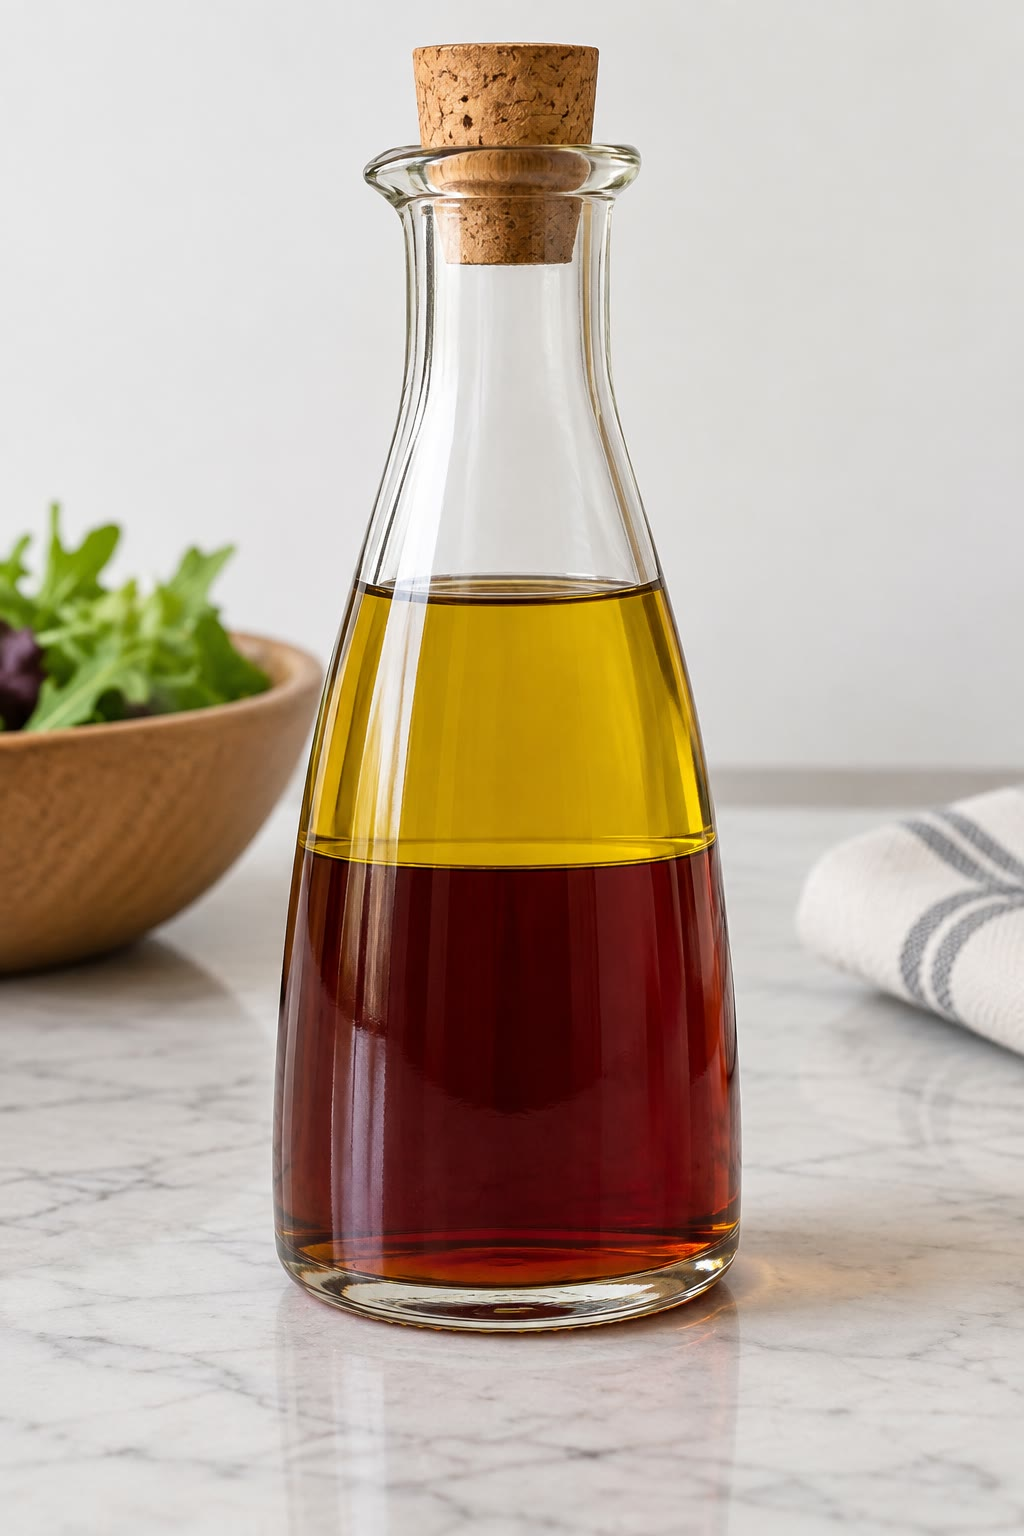
\includegraphics[width=0.2\linewidth]{images/book2/ai/b1-04-dressing.jpg}

{\small विश्राम में रखी सलाद ड्रेसिंग: अध्रुवीय जैतून का तेल सिरके पर तैरता है,
जो एक जलीय विलयन है; दोनों द्रव अमिश्रणीय हैं।}
\end{omfigure}

\begin{definition}[जलरागी, जलविरागी, उभयरागी]\label{def:b1:intermolecular-forces-solvents:amphiphile}
कोई समूह \emph{जलरागी}\index{जलरागी} होता है जब वह पानी के साथ
अनुकूल अन्योन्यक्रिया करता है (आयनिक या ध्रुवीय समूह: \ce{-COO^-}, \ce{-OH},
\ce{-SO3^-}) और \emph{जलविरागी}\index{जलविरागी} जब नहीं करता
(हाइड्रोकार्बन श्रृंखलाएँ)। कोई अणु \emph{उभयरागी}\index{उभयरागी} होता है
जब उस पर जलरागी शीर्ष और जलविरागी पूँछ दोनों हों।
\end{definition}

\begin{example}[साबुन]\label{ex:b1:intermolecular-forces-solvents:soap}
सोडियम डोडेकेनोएट, \ce{CH3(CH2)10COO- Na+}, \omterm{def:b1:intermolecular-forces-solvents:amphiphile}{उभयरागी} है। पानी की
सतह पर इसके अणु शीर्ष पानी में और पूँछ हवा में रखकर खड़े रहते हैं। पानी के भीतर,
एक छोटी सांद्रता से ऊपर, वे गोलों में इकट्ठे हो जाते हैं --- मिसेल --- जिनमें
पूँछें भीतर और शीर्ष बाहर होते हैं। अध्रुवीय चिकनाई
मिसेलों के \omterm{def:b1:intermolecular-forces-solvents:amphiphile}{जलविरागी} क्रोड में घुल जाती है और पानी के साथ बह जाती है।
\end{example}

\begin{omfigure}
\begin{tikzpicture}[font=\small]
  % interface
  \fill[omWater] (-3.2,-1.6) rectangle (-0.4,0);
  \draw[omDef!60] (-3.2,0) -- (-0.4,0);
  \node[anchor=south west] at (-3.2,0.95) {हवा};
  \node[anchor=north west] at (-3.2,-1.2) {पानी};
  \foreach \x in {-2.9,-2.5,...,-0.6} {
    \fill[omThm] (\x,-0.12) circle (0.11);
    \draw[thick, black!70, decorate, decoration={zigzag, amplitude=1pt, segment length=3pt}] (\x,0) -- (\x,0.85);
  }
  % micelle
  \begin{scope}[xshift=3.2cm, yshift=-0.4cm]
    \fill[omWater] (-2,-1.6) rectangle (2,1.6);
    \foreach \a in {0,30,...,330} {
      \draw[thick, black!70, decorate, decoration={zigzag, amplitude=1pt, segment length=3pt}] (\a:0.25) -- (\a:1.0);
      \fill[omThm] (\a:1.12) circle (0.11);
    }
    \node[anchor=north] at (0,-1.65) {पानी में एक मिसेल};
  \end{scope}
\end{tikzpicture}

{\small \omterm{def:b1:intermolecular-forces-solvents:amphiphile}{उभयरागी} अणु (लाल \omterm{def:b1:intermolecular-forces-solvents:amphiphile}{जलरागी} शीर्ष, टेढ़ी-मेढ़ी \omterm{def:b1:intermolecular-forces-solvents:amphiphile}{जलविरागी}
पूँछ) पानी की सतह पर और एक मिसेल में इकट्ठे, अनुप्रस्थ काट
में बने हुए; मिसेलों का अध्ययन तृतीय वर्ष के खंड में होता है।}
\end{omfigure}

\begin{method}[विलायक चुनना]\label{met:b1:intermolecular-forces-solvents:choose}
किसी विलेय या अभिक्रिया के लिए विलायक चुनने हेतु:
\begin{enumerate}
  \item विलेय का लक्षण पहचानिए: आयनिक, ध्रुवीय, \omterm{def:b1:intermolecular-forces-solvents:hbond}{हाइड्रोजन आबंध} देने या
        ग्रहण करने में समर्थ, या अध्रुवीय;
  \item उसी प्रकार का विलायक चुनिए (\cref{prop:b1:intermolecular-forces-solvents:like}),
        और यदि आयनों को अलग करना हो तो उच्च परावैद्युतांक वाला;
  \item किसी ऋणायन और किसी अणु के बीच अभिक्रिया के लिए ध्रुवीय
        \omterm{def:b1:intermolecular-forces-solvents:solvent-classes}{अप्रोटिक विलायक} को वरीयता दीजिए, जो लवण को घोलता है पर ऋणायन को
        \omterm{def:b1:intermolecular-forces-solvents:hbond}{हाइड्रोजन आबंधों} से नहीं बाँधता (\cref{ch:b1:nucleophilic-substitution});
  \item निष्कर्षण के लिए ऐसा विलायक चुनिए जो पहले विलायक के साथ अमिश्रणीय हो
        और जिसमें विलेय कहीं अधिक विलेय हो।
\end{enumerate}
\end{method}

\section{अभ्यास}

\begin{exercise}[$\star$]\label{exo:b1:intermolecular-forces-solvents:1}
द्रव आर्गन, द्रव हाइड्रोजन क्लोराइड, द्रव पानी, द्रव मेथेन और ठोस
डाइआयोडीन के कणों के बीच मौजूद अन्योन्यक्रियाओं के नाम बताइए, और हर एक में
कौन-सी प्रधान है, यह भी बताइए।
\end{exercise}

\begin{exercise}[$\star$]\label{exo:b1:intermolecular-forces-solvents:2}
इनमें से कौन-से पदार्थ अपने ही अणुओं के बीच \omterm{def:b1:intermolecular-forces-solvents:hbond}{हाइड्रोजन आबंध} बनाते हैं:
\ce{CH3OH}, \ce{CH3OCH3}, \ce{CH3NH2}, \ce{CH3F}, \ce{HF},
\ce{CH4}? कौन-से किसी दूसरे अणु से केवल \omterm{def:b1:intermolecular-forces-solvents:hbond}{हाइड्रोजन आबंध} ग्रहण कर सकते हैं?
\end{exercise}

\begin{exercise}[$\star$]\label{exo:b1:intermolecular-forces-solvents:3}
विलायकों की सारणी की सहायता से पानी, एथेनॉल, प्रोपेनोन, हेक्सेन,
डाइक्लोरोमेथेन और ऐसीटोनाइट्राइल को ध्रुवीय या अध्रुवीय, प्रोटिक या अप्रोटिक में वर्गीकृत कीजिए।
\end{exercise}

\begin{exercise}[$\star$]\label{exo:b1:intermolecular-forces-solvents:4}
समझाइए कि डाइआयोडीन पानी की तुलना में हेक्सेन में कहीं बेहतर क्यों घुलता है, और
सोडियम क्लोराइड इसका उलटा क्यों करता है।
\end{exercise}

\begin{exercise}[$\star\star$]\label{exo:b1:intermolecular-forces-solvents:5}
मेथेनॉल \qty{64.7}{\celsius} पर उबलता है, एथेनॉल \qty{78.4}{\celsius} पर,
एथेनोइक अम्ल \qty{118.1}{\celsius} पर और मेथॉक्सीमेथेन
\qty{-25.0}{\celsius} पर। इस क्रम की व्याख्या कीजिए।
% ledger: bp:CH3OH, bp:C2H5OH, bp:CH3COOH, bp:CH3OCH3
\end{exercise}

\begin{exercise}[$\star\star$]\label{exo:b1:intermolecular-forces-solvents:6}
निर्वात में \qty{500}{pm} दूर स्थित एक \ce{Na+} और एक \ce{Cl-} आयन के बीच कूलॉम बल
परिकलित कीजिए ($\varepsilon_0 = \qty{8.854e-12}{F/m}$,
$e = \qty{1.602e-19}{C}$), फिर पानी में ($\varepsilon_r = 78.4$) और
हेक्सेन में ($\varepsilon_r = 1.89$)। टिप्पणी कीजिए।
\end{exercise}

\begin{exercise}[$\star\star$]\label{exo:b1:intermolecular-forces-solvents:7}
प्रोपेनोन और पानी सभी अनुपातों में \omterm{def:b1:intermolecular-forces-solvents:miscibility}{मिश्रणीय} हैं; हेक्सेन और पानी
नहीं। टूटने और बनने वाली अन्योन्यक्रियाओं पर विचार करके समझाइए।
\end{exercise}

\begin{exercise}[$\star\star$]\label{exo:b1:intermolecular-forces-solvents:8}
\ce{HCl} का \omterm{def:b1:lewis-resonance-vsepr:dipole}{द्विध्रुव आघूर्ण} \qty{1.09}{\debye} है और वह
\qty{-85.0}{\celsius} पर उबलता है; \ce{HBr} का \qty{0.83}{\debye} है और वह
\qty{-66.4}{\celsius} पर उबलता है। कम \omterm{def:b1:lewis-resonance-vsepr:dipole}{ध्रुवीय अणु} ऊँचे ताप पर क्यों उबलता है?
% ledger: dip:HCl, dip:HBr, bp:HCl, bp:HBr
\end{exercise}

\begin{exercise}[$\star\star$]\label{exo:b1:intermolecular-forces-solvents:9}
एथेनोइक अम्ल का चक्रीय द्वितय बनाइए। बेंज़ीन विलयन में एथेनोइक
अम्ल ऐसा व्यवहार करता है मानो उसका मोलर द्रव्यमान \qty{60}{g/mol} का लगभग दोगुना हो; पानी
में नहीं। दोनों तथ्यों की व्याख्या कीजिए।
\end{exercise}

\begin{exercise}[$\star\star\star$]\label{exo:b1:intermolecular-forces-solvents:10}
पानी में सोडियम क्लोराइड के घुलने का वर्णन वियोजन और \omterm{def:b1:intermolecular-forces-solvents:dissolution}{विलायकन} के रूप में
कीजिए, और पानी में हाइड्रोजन क्लोराइड के घुलने का वर्णन आयनन, वियोजन और
\omterm{def:b1:intermolecular-forces-solvents:dissolution}{विलायकन} के रूप में। हेक्सेन में हाइड्रोजन क्लोराइड अचालक विलयन
क्यों देता है?
\end{exercise}

\begin{exercise}[$\star\star\star$]\label{exo:b1:intermolecular-forces-solvents:11}
रैखिक ऐल्केनों के क्वथनांकों से (पेंटेन
\qty{36.1}{\celsius}, डेकेन \qty{174.1}{\celsius}) प्रति \ce{CH2} समूह औसत वृद्धि,
\ce{C5} और \ce{C10} के बीच, परिकलित कीजिए, और अनडेकेन के
क्वथनांक का अनुमान लगाइए। श्रेणी में आगे बढ़ने पर वृद्धि क्यों घटती है?
% ledger: bp:C5H12, bp:C10H22
\end{exercise}

\begin{exercise}[$\star\star\star$]\label{exo:b1:intermolecular-forces-solvents:12}
सोडियम डोडेसिल सल्फ़ेट, \ce{CH3(CH2)11OSO3^- Na+}, एक अपमार्जक है। इसके
\omterm{def:b1:intermolecular-forces-solvents:amphiphile}{जलरागी} और \omterm{def:b1:intermolecular-forces-solvents:amphiphile}{जलविरागी} भाग पहचानिए, पानी की सतह पर और एक मिसेल में इसकी
व्यवस्था का रेखाचित्र बनाइए, और समझाइए कि यह कपड़े से तेल का
धब्बा कैसे हटाता है।
\end{exercise}

\section{समस्या: यदि पानी में हाइड्रोजन आबंध न होते}

\begin{problem}[{सप्ताहांत समस्या --- उत्कृष्ट गैसों और ऐल्केनों में लंदन बल,
विलायक का चुनाव, और वह क्वथनांक जो हाइड्रोजन आबंधों के बिना पानी का
होता}]
\label{pb:b1:intermolecular-forces-solvents:1}
\qty{1}{atm} पर क्वथनांक (\unit{\celsius} में): \ce{He} $-268.9$,
\ce{Ne} $-246.1$, \ce{Ar} $-185.9$, \ce{Kr} $-153.4$, \ce{Xe} $-108.1$;
पेंटेन 36.1, हेक्सेन 68.8; \ce{CH4} $-161.5$, \ce{SiH4} $-112.0$,
\ce{GeH4} $-88.1$; \ce{NH3} $-33.4$, \ce{PH3} $-87.8$, \ce{AsH3} $-62.5$;
\ce{H2O} 100.0, \ce{H2S} $-60.3$, \ce{H2Se} $-41.3$; \ce{HF} 19.6,
\ce{HCl} $-85.0$, \ce{HBr} $-66.4$।
% ledger: bp:He, bp:Ne, bp:Ar, bp:Kr, bp:Xe, bp:C5H12, bp:C6H14, bp:CH4,
% bp:SiH4, bp:GeH4, bp:NH3, bp:PH3, bp:AsH3, bp:H2O, bp:H2S, bp:H2Se,
% bp:HF, bp:HCl, bp:HBr

\medskip
\noindent\textbf{भाग I --- केवल लंदन।}
\begin{enumerate}
  \item द्रव आर्गन के परमाणुओं को कौन-सी अन्योन्यक्रिया जोड़े रखती है?
  \item हीलियम से ज़ेनॉन तक क्वथनांक की वृद्धि समझाइए।
  \item हीलियम का क्वथनांक सभी पदार्थों में सबसे कम क्यों है?
  \item पेंटेन और हेक्सेन की तुलना कीजिए: एक \ce{CH2} समूह क्या जोड़ता है?
  \item मेथेन, सिलेन और जर्मेन का कोई \omterm{def:b1:lewis-resonance-vsepr:dipole}{द्विध्रुव आघूर्ण} नहीं है। कौन-सी
        अन्योन्यक्रिया उनके क्वथनांकों के क्रम की व्याख्या करती है?
  \item मेथेन में कोई \omterm{def:b1:intermolecular-forces-solvents:hbond}{हाइड्रोजन आबंध} संभव क्यों नहीं है?
\end{enumerate}

\medskip
\noindent\textbf{भाग II --- विलायक चुनना।}
अध्याय की विलायकों की सारणी का उपयोग कीजिए।
\begin{enumerate}[resume]
  \item सारणी का कौन-सा विलायक सोडियम क्लोराइड को सबसे अच्छी तरह घोलता है, और
        क्यों?
  \item समान दूरी पर दो आयनों के बीच का आकर्षण हेक्सेन की तुलना में पानी में
        कितने गुना कम है?
  \item ऋणायन \ce{CN-} और किसी कार्बनिक अणु के बीच अभिक्रिया ऐसे विलायक में
        की जानी चाहिए जो लवण को घोले पर ऋणायन को \omterm{def:b1:intermolecular-forces-solvents:hbond}{हाइड्रोजन आबंधों} से
        न बाँधे। एक चुनिए।
  \item जलीय विलयन से डाइआयोडीन निकालने के लिए आप सारणी का कौन-सा
        विलायक चुनेंगे, और आयोडीन किस परत में पहुँचेगा?
  \item समझाइए कि उस निष्कर्षण के लिए एथेनॉल का उपयोग क्यों नहीं किया जा सकता।
  \item एथॉक्सीएथेन ध्रुवीय होने पर भी पानी के साथ बहुत कम \omterm{def:b1:intermolecular-forces-solvents:miscibility}{मिश्रणीय} है।
        एक व्याख्या प्रस्तावित कीजिए।
\end{enumerate}

\medskip
\noindent\textbf{भाग III --- अन्य हाइड्राइड।}
\begin{enumerate}[resume]
  \item \omterm{def:b1:periodicity:table}{समूह} 17 के लिए \ce{HCl} से
        \ce{HBr} तक क्वथनांक का परिवर्तन परिकलित कीजिए, और उसी परिवर्तन को पीछे \omterm{def:b1:periodicity:table}{आवर्त} 2 तक बहिर्वेशित कीजिए।
  \item बहिर्वेशित मान की तुलना \ce{HF} के क्वथनांक से कीजिए।
  \item यही दो प्रश्न \omterm{def:b1:periodicity:table}{समूह} 15 के लिए (\ce{PH3}, \ce{AsH3} और
        \ce{NH3})।
  \item \omterm{def:b1:periodicity:table}{समूह} 14 के लिए, क्या \ce{CH4}, \ce{SiH4} और \ce{GeH4} से किए गए
        बहिर्वेशन के ऊपर है या नीचे? यह आश्चर्यजनक क्यों नहीं है?
  \item \ce{NH3}, \ce{HF} और पानी के आधिक्यों को क्रम में रखिए।
  \item \ce{NH3}, \ce{HF} और
        \ce{H2O} का हर अणु कितने \omterm{def:b1:intermolecular-forces-solvents:hbond}{हाइड्रोजन आबंध} दे और ले सकता है, यह गिनिए, और क्रम की व्याख्या कीजिए।
\end{enumerate}

\medskip
\noindent\textbf{भाग IV --- \omterm{def:b1:intermolecular-forces-solvents:hbond}{हाइड्रोजन आबंधों} के बिना पानी।}
\begin{enumerate}[resume]
  \item \ce{H2S} और \ce{H2Se} बहिर्वेशन के लिए उपयुक्त क्यों हैं, और
        स्वयं पानी क्यों नहीं?
  \item \ce{H2S} से \ce{H2Se} तक क्वथनांक का परिवर्तन परिकलित कीजिए।
  \item इन दो बिंदुओं से गुज़रने वाली सरल रेखा का समीकरण लिखिए,
        \omterm{def:b1:periodicity:table}{आवर्त} $p$ को चर लेकर।
  \item $p = 2$ पर पानी का जो क्वथनांक होता, वह निकालिए।
  \item \omterm{def:b1:intermolecular-forces-solvents:hbond}{हाइड्रोजन आबंध} पानी का क्वथनांक कितना बढ़ाते हैं?
  \item निष्कर्ष निकालिए: यदि पानी के अणु एक-दूसरे को \ce{H2S} के अणुओं की तरह
        आकर्षित करते, तो पानी किस ताप पर उबलता?
\end{enumerate}
\end{problem}
